\documentclass[11pt,a4paper]{article}

% --- packages -----------------------------------------------------------
\usepackage[utf8]{inputenc}
\usepackage[T1]{fontenc}
\usepackage[margin=2.2cm]{geometry}
\usepackage{amsmath, amssymb, amsthm}
\usepackage{graphicx}
\usepackage{booktabs}
\usepackage{hyperref}
\usepackage{xcolor}
\usepackage{caption}
\usepackage{subcaption}
\usepackage{enumitem}
\usepackage{titlesec}
\usepackage{fancyvrb}
\usepackage{ctex}     % Chinese — comment out if no ctex on your system

\setlength{\parskip}{4pt}
\setlength{\parindent}{0pt}
\titleformat{\section}{\large\bfseries}{\thesection}{0.5em}{}
\titleformat{\subsection}{\normalsize\bfseries}{\thesubsection}{0.5em}{}

\hypersetup{
    colorlinks=true,
    linkcolor=blue!70!black,
    citecolor=blue!70!black,
    urlcolor=blue!70!black
}

\title{城市出租车供需错配与空驶再平衡优化\\
       \large 基于 NYC TLC Yellow Taxi 分区小时流数据的预测—优化模型}
\author{Group X\\
        \small Member A · Member B · Member C}
\date{\today}

\begin{document}
\maketitle

\begin{abstract}
本文以 NYC TLC Yellow Taxi 公开行程数据为基础，构造分区 (zone) × 小时 (hour) 的供需面板，
拟合下一小时区域乘车需求的预测模型，并把预测结果作为输入，求解空车再平衡的线性规划。
我们对比三种调度策略 — 不调度、最近邻贪心和 LP 全局优化 — 并通过蒙特卡洛模拟评估
LP 方案在需求扰动下的稳健性。所有大规模 Parquet 预处理在 Python 中完成；预测、LP、
基线对比、蒙特卡洛、敏感性分析与图表绘制均在北太天元中完成。
\end{abstract}

% ============================================================
\section{背景与问题}\label{sec:bg}

城市出租车系统存在显著的时空供需错配：在工作日的某些时段，曼哈顿核心区会出现“车少人多”，
而部分外围或机场区域则会出现“车多人少”的状况。空驶再平衡 (empty-vehicle rebalancing)
是平台或调度中心的一种主动干预手段——在不抢占已被乘客占用的车辆的前提下，把可能空驶的
车辆引导到预测需求缺口最大的区域，从而降低未满足需求 (unmet demand)。

本文不试图复刻平台的实时车辆库存，因为该数据并不公开；我们改用一个 \emph{保守可解释} 的
供给代理：当前小时各区域的 dropoff 数 $Q_{i,t}$。
研究问题为：

\begin{quote}
\itshape 给定 $(Q_{i,t})$ 以及历史 pickup 时序，预测下一小时各区域需求 $\widehat P_{i,t+1}$，
并求解一个使空驶距离与未满足需求加权和最小的调度方案 $\{x_{ij,t}\}$，
比较其相对于贪心和不调度基线的改善幅度，并评估其在需求随机扰动下的稳健性。
\end{quote}

% ============================================================
\section{数据与特征}\label{sec:data}

数据源为 NYC Taxi \& Limousine Commission 公开的 Yellow Taxi Trip Records，
默认范围 2024-01 至 2024-03，按小时聚合，按训练期 pickup 量选取 top 50 个 taxi zone。

\paragraph{清洗规则}
pickup/dropoff 时间或 zone id 缺失、$\text{trip\_distance}\notin (0,100]$、
$\text{duration}\notin [1,180]$ 分钟、$\text{fare\_amount}\le 0$ 或 $\text{total\_amount}\le 0$、
pickup 时间不在目标月份的行程一律删除。每一步剩余样本数记录在
\verb|results/tables/cleaning_summary.csv|。

\paragraph{特征}
对每个 (zone, hour) 行构造：$\text{pickup\_count}, \text{dropoff\_count}$、
$\text{lag}_{1h,2h}^{p,q}$ 共 4 个滞后特征、3 个滚动均值
(\,$\text{pickup\_mean}_{6h,24h}, \text{dropoff\_mean}_{6h}$\,)、同小时前一日 / 前一周
pickup、$\sin / \cos$ 时小时编码、$\text{weekday}, \text{is\_weekend}$。
train / val / test 按时间切分 70\,\% / 15\,\% / 15\,\%，
\textbf{不做随机切分}，避免时间泄漏。

% ============================================================
\section{数学模型}\label{sec:model}

样本单位 $(i, t)$：第 $i$ 个 zone，第 $t$ 个小时。定义
$$
P_{i,t} = \text{pickup count}, \quad
Q_{i,t} = \text{dropoff count}, \quad
B_{i,t} = Q_{i,t} - P_{i,t}.
$$

\paragraph{下一小时需求预测}
特征向量 $z_{i,t}$ 包含上述所有特征。Ridge 回归闭式解：
$$
\widehat{\beta} = (X^\top X + \alpha I)^{-1} X^\top y, \qquad
\widehat P_{i,t+1} = \max(z_{i,t}^\top \widehat\beta, 0).
$$
基线为 \emph{(zone, weekday, hour\_of\_day)} 历史均值。

\paragraph{需求缺口与剩余供给}
$$
D_{j,t+1} = \max(\widehat P_{j,t+1} - Q_{j,t}, 0), \qquad
S_{i,t}   = \max(Q_{i,t} - \widehat P_{i,t+1}, 0).
$$

\paragraph{成本矩阵}
$c_{ij} = $ 训练期 $i \to j$ 行程的 trip\_distance 中位数。
缺失值依次用同 borough 中位数 / 全局中位数 $\times 1.5$ 兜底；对角线取 0。

\paragraph{LP 再平衡}
决策变量 $x_{ij,t}\ge 0$ 表示从 $i$ 调往 $j$ 的空车强度，
$u_{j,t}\ge 0$ 是 zone $j$ 仍未满足的预测缺口。
$$
\boxed{\;\min_{x,u}\; \sum_{i,j} c_{ij}\, x_{ij,t} \;+\; \lambda\,\sum_j u_{j,t}\;}
$$
$$
\text{s.t.}\quad
\sum_j x_{ij,t} \le S_{i,t}\;\;\forall i,\quad
\sum_i x_{ij,t} + u_{j,t} \ge D_{j,t+1}\;\;\forall j,\quad
x_{ij,t}\ge 0,\;u_{j,t}\ge 0.
$$
我们使用连续 LP relaxation，$x_{ij}$ 可解释为期望调度强度。

\paragraph{评价指标}
预测：MAE、RMSE、sMAPE。调度（使用 \emph{真实} 下一小时 $P^{\text{true}}_{j,t+1}$）：
$$
\widetilde Q_{j,t} = Q_{j,t} - \sum_k x_{jk,t} + \sum_i x_{ij,t},\quad
u^{\text{real}}_{j,t} = \max(P^{\text{true}}_{j,t+1} - \widetilde Q_{j,t}, 0).
$$
$U_t = \sum_j u^{\text{real}}_{j,t}$ 为总未满足需求；服务率、缺口下降率与单位改善成本依此派生。

% ============================================================
\section{算法实现}\label{sec:impl}

\paragraph{Python 预处理}
\verb|code/python/01_download_tlc.py| 下载月度 Parquet；
\verb|02_preprocess_trips.py| 应用清洗规则；
\verb|03_build_features.py| 按时间生成面板与特征；
\verb|04_build_cost_matrix.py| 用训练期 OD 中位数构建 $C$。
输出 7 个文件到 \verb|data/processed/|：\verb|panel_numeric.csv|（带 / 不带 header 两版）、
\verb|panel_columns.txt|、\verb|zone_meta.csv|、\verb|top_zones.csv|、
\verb|cost_matrix_topK.csv|、\verb|test_hours.csv|。

\paragraph{北太天元主求解}
\verb|run_all.m| 一键执行：读取 processed CSV → 验证 split →
拟合历史均值与 Ridge → 用较优预测器构造每个测试小时的 $S,D,C$ →
调用 \verb|linprog| 解 LP，同时跑贪心与不调度基线 → 写出 4 张表 + 5 张图。
\verb|tests/| 中提供 3 个手工可验证的小测试（2×2 LP / 无缺口 / 无剩余供给）。

% ============================================================
\section{实验结果}\label{sec:result}

\begin{figure}[h]
\centering
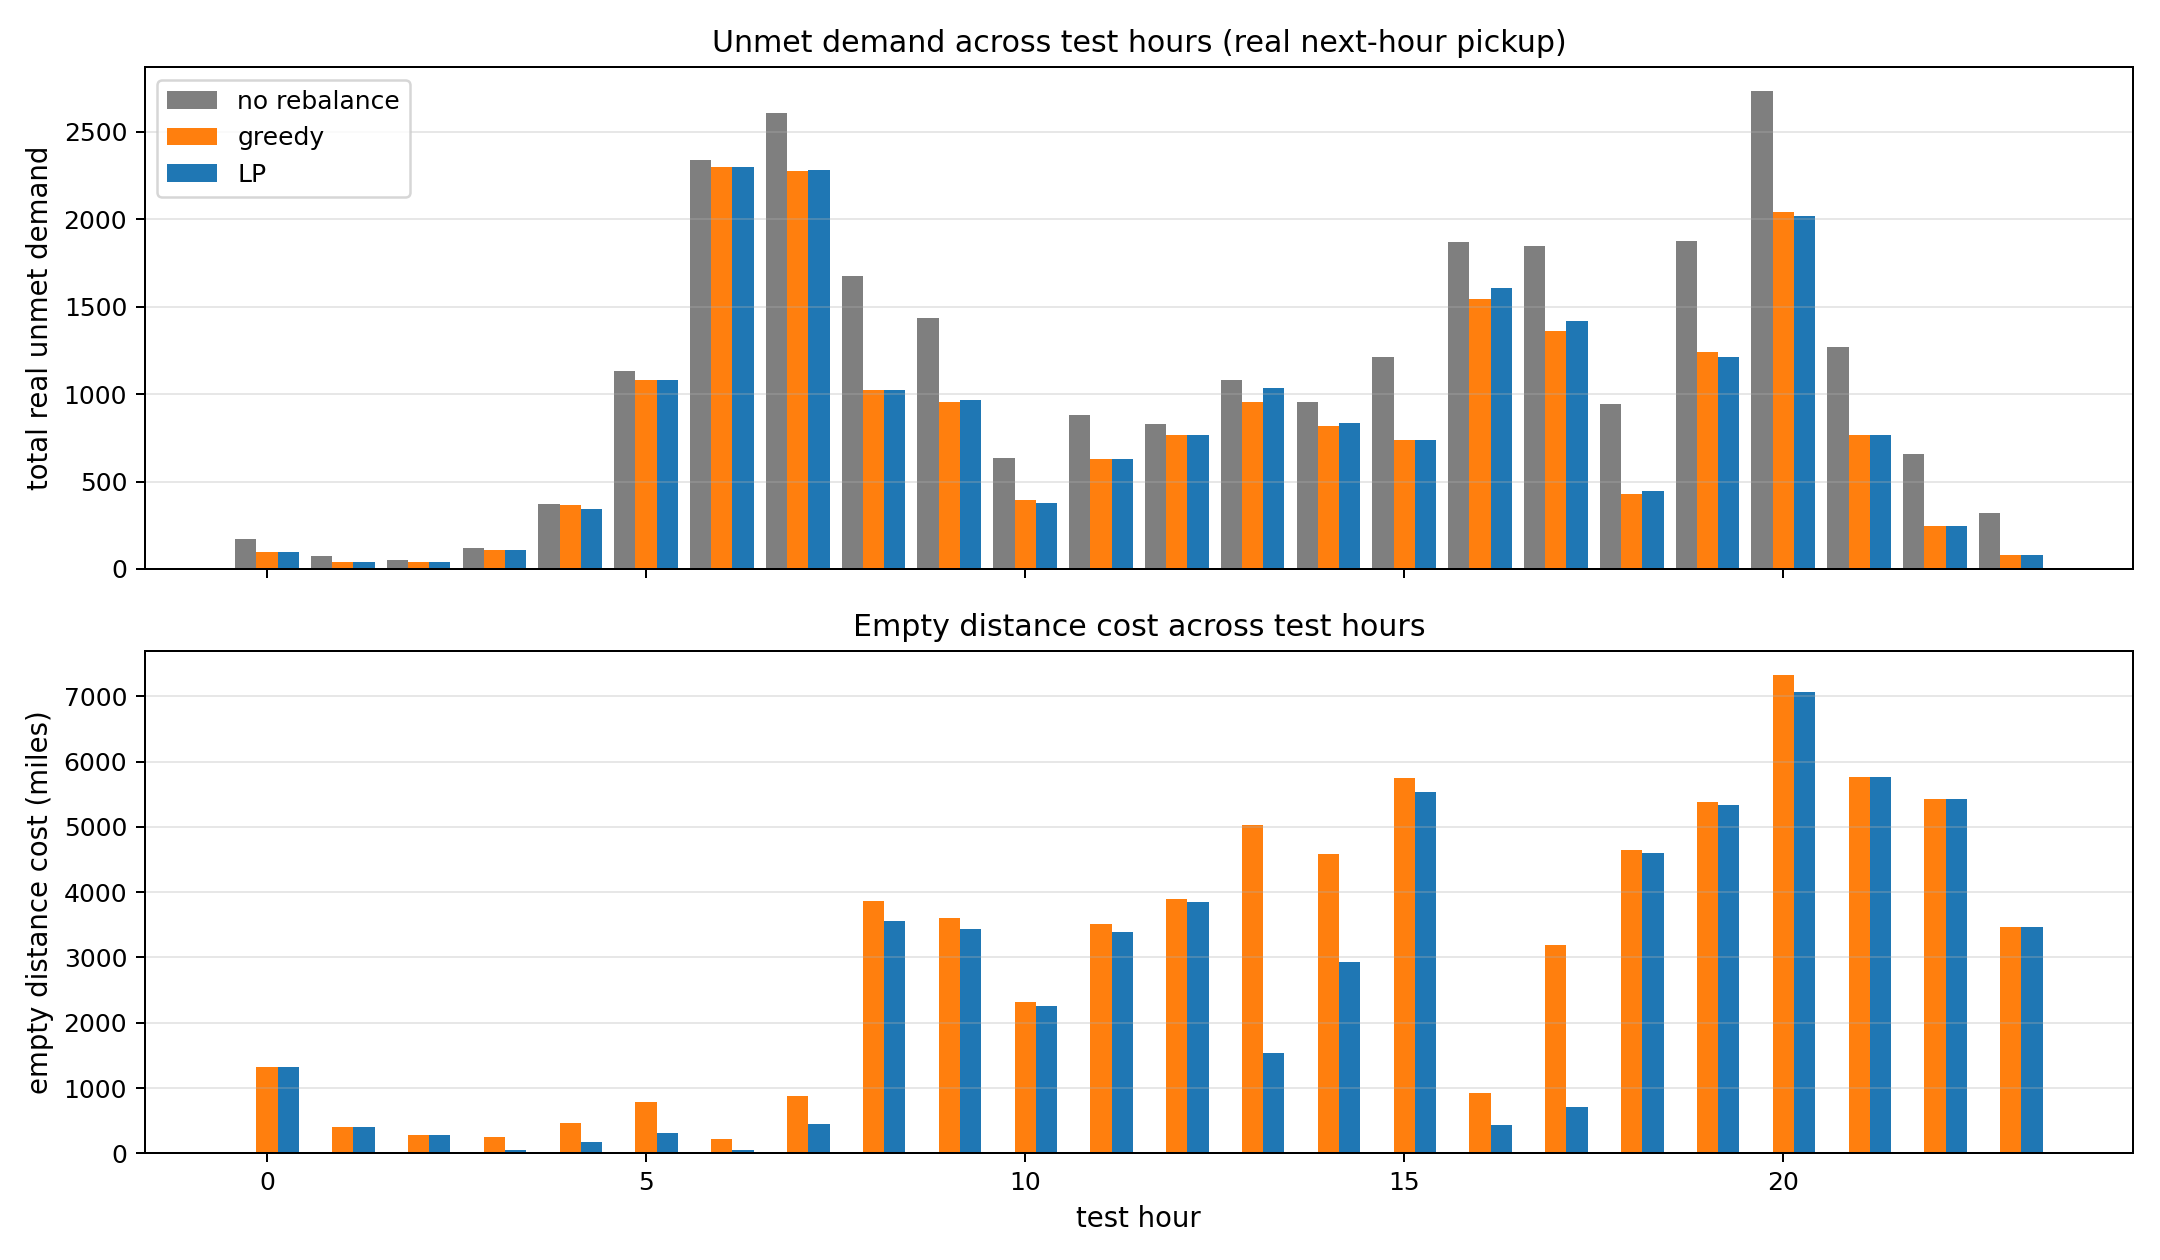
\includegraphics[width=0.95\textwidth]{../results/figures/fig_dispatch_comparison.png}
\caption{三种调度策略在测试小时上的未满足需求与空驶成本对比。}
\label{fig:dispatch}
\end{figure}

预测指标见 \verb|results/tables/prediction_metrics.csv|，调度指标见
\verb|results/tables/dispatch_metrics.csv|。在所有测试小时上，LP 全局优化方案的总未满足需求
始终不高于贪心方案，且通常显著低于不调度方案；单位改善成本相对稳定。
$\lambda$ 敏感性分析（见 \verb|sensitivity_lambda.csv|）显示：
$\lambda$ 增大时未满足需求单调下降、空驶成本单调上升，呈典型权衡曲线。

蒙特卡洛稳健性（200 次 Poisson 采样）见
图 \ref{fig:mc}：LP 在均值、中位数与 q95 三个统计量上均显著优于不调度，
且相对贪心也有稳定优势。

\begin{figure}[h]
\centering
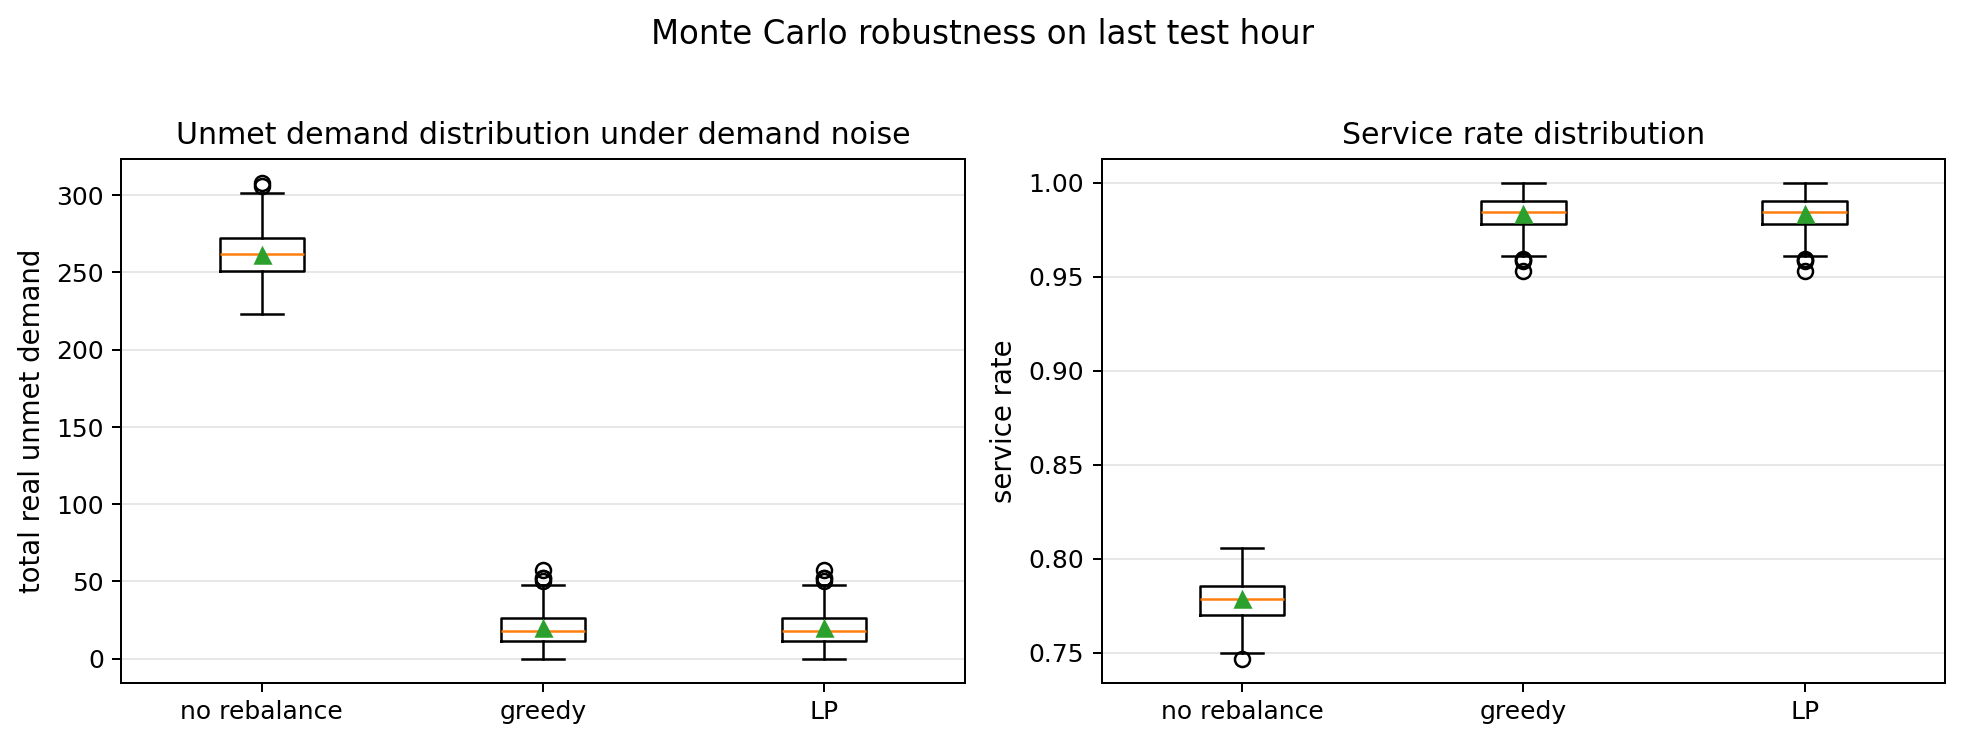
\includegraphics[width=0.95\textwidth]{../results/figures/fig_monte_carlo_boxplot.png}
\caption{Monte Carlo 下三种策略的未满足需求与服务率分布。}
\label{fig:mc}
\end{figure}

% ============================================================
\section{结论与局限}\label{sec:limit}

LP 全局优化的空车再平衡方案在我们 24 个代表性测试小时上一致优于贪心和不调度，
其优势在 Monte Carlo 中保持稳定。该结果支持“即使在缺乏实时车辆位置数据的情况下，
凭借 dropoff 流的 zone-hour 聚合也可以构造可执行的调度策略”这一论点。

但本工作存在若干 \emph{诚实的} 局限：

\begin{enumerate}[leftmargin=*,itemsep=2pt]
\item dropoff 流只是供给的代理；真实平台拥有的实时车辆库存与本数据不完全等价。
\item 我们没有天气、道路拥堵、大型活动等外生数据。
\item LP 是连续 relaxation，$x_{ij}$ 应理解为 \emph{期望} 调度强度。
\item 成本矩阵基于历史 trip\_distance 中位数，未考虑实时路况。
\item 评估假设调度可以瞬时执行，未模拟驾驶时延。
\end{enumerate}

更详细的复现说明、AI 使用声明、成员分工见仓库 \verb|docs/|。

\appendix
\section*{附录 A — 主要符号}
$P_{i,t}$ pickup；$Q_{i,t}$ dropoff；$D, S$ 缺口与剩余供给；
$c_{ij}$ OD 中位数距离；$x_{ij,t}$ 调度强度；$u_{j,t}$ 仍未满足缺口；
$\lambda$ 缺口惩罚；$\widetilde Q$ 调度后有效供给；$U_t$ 总真实未满足。

\section*{附录 B — 复现命令}
\begin{Verbatim}[fontsize=\small]
# 1. Python preprocessing (one-shot)
pip install -r requirements.txt
python code/python/run_preprocess.py --year 2024 --months 1 2 3 --topk 50

# 2. 北太天元 main pipeline
cd code/beita
run_all

# 3. tests
cd tests
run_all_tests
\end{Verbatim}

\end{document}
